\chapter{Model Extensions}
The prime objective of this chapter is to extend the event-driven model of Chapter \ref{chpt:ED} in two different ways. On one hand, in Section \ref{sec:GBM} the risky asset is modeled in a continuous-time setting by employing the theory of \gls{GBM}; on the other hand, in Section \ref{sec:Interest_rate_dynamics} we no longer let the risk-free asset evolve deterministically but instead its short-rate will evolve according to the Vasicek model. Throughout the chapter, the trade-off between a more detailed model and the increase in computational complexity will be evident.
\section{A GBM dynamics for the risky asset}\label{sec:GBM}
Let us consider the same portfolio as in Chapter \ref{chpt:ED}, namely a risky and a risk-free asset. As far as the risk-free asset is concerned, the deterministic model of Chapter \ref{chpt:ED} remains unchanged. On the other hand, the following dynamics for the risky asset is assumed
\[
\begin{cases*}
dS_t  = \mu S_t dt + \sigma S_t dW_t\\
S_{t_k} = S_k, \quad t\geq t_k
\end{cases*}
\]
where $\{W_t\}_{t\geq t_k}$ is a unidimensional Brownian motion and $t_k$ the time when the k-th event occurs. Solving the above \gls{SDE} brings 
\begin{align*}
S_t & = S_k \exp\big\{(\mu-\sigma^2/2)(t-t_k)+\sigma(W_t-W_{t_k})\}\\
& = S_k \exp\big\{\widetilde{\mu}(t-t_k)+\sigma(W_t-W_{t_k})\}
\end{align*}
where we defined $\widetilde{\mu}= \mu-\sigma^2/2$. The cumulative risky asset log-return (starting from $t_k$) is denoted by $\{X_t\}_{t\geq t_k}$ and is equal to
\begin{equation}
X_t = \log\big(S_t/S_{t_k}\big)=\widetilde{\mu}(t-t_k) + \sigma(W_t-W_{t_k}).
\end{equation}
Given that in the development of the model it will be more convenient to have the time starting from 0, exploiting the Translation Invariance property of Brownian motion we define the translated log-return process as follows
\begin{equation}\label{eq:translatedGBM}
\widetilde{X}_t = X_{t+t_k} = \widetilde{\mu}t + \sigma(W_{t+t_k}-W_{t_k}) = \widetilde{\mu}t + \sigma \widetilde{W}_t \quad t\geq 0.
\end{equation}
In this case $t$ represents the interevent time instead of the elapsed time.
\subsection{The double exit problem }
In the event-driven setting introduced in the previous chapter, what triggers a portfolio rebalancing is the fact that the absolute value of process $\widetilde{X}_t$ exceeds $J$. When this happens, we say, in the event-driven jargon, that an event has occurred. Therefore, it is of prime interest  modeling the stochastic time instant when the next event takes place. This could be done by defining the following stopping time
\begin{align}\label{eq:stopping_time}
\tau_{k+1} & = \inf\big\{t\geq 0 \colon \lvert\widetilde{X}_t\lvert\geq J \big\}\\\nonumber
& = \inf\big\{t\geq 0 \colon \widetilde{X}_t \notin (-J,J) \big\}.
\end{align}
Given that eventually the density function of $x_{k+1}$ will be needed, we are interested in the distribution of random variable (\ref{eq:stopping_time}). This problem is known in literature as \textit{the double exit problem of a Brownian motion with drift}. The central result is given by the following theorem, which covers a more general case in which the upper and lower barrier are different. The theorem is taken from \cite{Hieber2012} as is.
\begin{theorem}[double exit problem]\label{thm:double_exit_problem}
	Let $X_t = \mu t + \sigma W_t$ be a Brownian motion with drift, $\mu \in \mathbb{R}$ and $\sigma > 0$. Moreover, assume there are two constant barriers $b<0<a$. The distribution of $\tau = \inf\big\{t\geq 0 \colon X_t \notin (b,a) \big\}$ is 
	\[
	F_{\tau}(t) = 1-\bigg(\exp\Big\{\frac{\mu b}{\sigma^2}\Big\}K_T^{\infty}(a)-\exp\Big\{\frac{\mu a}{\sigma^2}\Big\}K_T^{\infty}(b) \bigg)
	\]
	where
	\[
	K_T^N(k)= \frac{\sigma^2\pi}{(a-b)^2}\sum_{n=1}^{N}\frac{n(-1)^{n+1}}{\frac{\mu^2}{2\sigma^2}+\frac{\sigma^2n^2\pi^2}{2(a-b)^2}}\exp\bigg\{-\bigg(\frac{\mu^2}{2\sigma^2}+\frac{\sigma^2n^2\pi^2}{2(a-b)^2}\bigg)t\bigg\}\sin\Big(\frac{n\pi k}{a-b}\Big).
	\]
	Applying the theorem to our case ($a=J, b=-J$) we get 
	\begin{equation}
	F_{\tau_{k+1}}(t)=1-\bigg[2\cosh\Big(\frac{\widetilde{\mu}J}{\sigma^2}\Big)K_t^{\infty}(J)\bigg]
	\end{equation}
	where we used the fact that $K_t^N(k)$ is odd as a function of $k$.
\end{theorem}

\subsection{Portfolio dynamics and the density of $x_{k+1}$}
Following the same path of Chapter \ref{chpt:ED}, we are left to compute the event-driven portfolio dynamics and it density function. As far as the first issue is concerned, the dynamics can be written as follows
\begin{equation}\label{eq:GBM_portfolio_dynamics}
\boxed{x_{k+1}=x_k\big(\exp\{r\tau_{k+1}\} + u_k\widetilde{X}_{\tau_{k+1}}\big)} \qquad k \in \mathbb{N}
\end{equation}
where $r$ is the risk-free asset constant return, $\tau_{k+1}$ is the stopping time (\ref{eq:stopping_time}), $u_k$ is the risky asset portfolio weight and $\widetilde{X}_{\tau_{k+1}}$ is the return process computed at the random time $\tau_{k+1}$. $\widetilde{X}_{\tau_{k+1}}$ can only assume the value $J$ or $-J$, therefore it is a Bernoullian random variable. Its parameter $p$ is given in the following lemma (which closely follows exercise 5.20 in \cite{baldi2017})
\begin{lemma}\label{lemma:probability_positive_jump}
	Let $\widetilde{X}_t$ be the return process (\ref{eq:translatedGBM}) and $\tau_{k+1}$ the stopping time in (\ref{eq:stopping_time}). Then $\widetilde{X}_{\tau_{k+1}} \sim B(p)$ where 
	\begin{align}
	p &= \mathbb{P}\Big(\widetilde{X}_{\tau_{k+1}}=J\Big)\\[2ex]\nonumber
	&=\frac{1-\exp\{2\widetilde{\mu}J/\sigma^2\}}{\exp\{-2\widetilde{\mu}J/\sigma^2\} - \exp\{2\widetilde{\mu}J/\sigma^2\}} \\[2ex]\nonumber
	& = \frac{\exp\{2\widetilde{\mu}J/\sigma^2\}-1}{2\sinh(2\widetilde{\mu}J/\sigma^2)}.
	\end{align}
\end{lemma}
\begin{proof}
	The first step of the proof consists in finding $\xi \in \mathbb{R}\setminus\{0\}$ such that $M=\exp\{\xi \widetilde{X}_t\}$ is a martingale. To this end, we apply Ito's formula (\cite{baldi2017}, Theorem 8.1) to $M_t$:
	\begin{align}\label{eq:Mt_dynamics}
	\nonumber
	dM_t & = \xi M_t d\widetilde{X}_t+\frac{1}{2}\xi^2M_t\sigma^2dt\\
	     & = \Big(\widetilde{\mu}\xi + \frac{1}{2}\sigma^2\xi^2\Big)M_t dt + \sigma\xi M_t \widetilde{W}_t.
	\end{align}
	If the drift in (\ref{eq:Mt_dynamics}) is null then $\{M_t\}_{t\geq0}$ is a martingale. Therefore, we impose the condition $\widetilde{\mu}\xi + \frac{1}{2}\sigma^2\xi^2 = 0$ which brings $ \xi = -2\widetilde{\mu}/\sigma^2$.
	
	The second part of the proof starts by noticing that also the process $\{M_{t\wedge\tau}\}_{t\geq 0}$ is a martingale\footnote{for the sake of clarity, we dropped the subscript $k+1$ from $\tau_{k+1}$}(\cite{baldi2017},Proposition 5.6). Moreover, since$\lvert M_{t\wedge\tau} \lvert \leq J$ for every $t\geq0$, we can apply the Dominated Convergence Theorem (\cite{baldi2017}, Proposition 4.2) in the following way:
	\begin{align*}
	\mathbb{E}\big[M_{\tau}\big] & = \mathbb{E}\Big[\lim\limits_{t\to\infty}M_{t\wedge\tau}\Big] = & (\text{Dominated Conv. Theorem})\\[2ex]
	& = \lim\limits_{t\to\infty}\underbrace{\mathbb{E}\big[M_{t\wedge\tau}\big]}_{1}=\\
	& = 1
	\end{align*}
	hence
	\begin{align*}
	\mathbb{E}\big[M_{\tau}\big] & = \exp\{2\widetilde{\mu}J/\sigma^2\}\mathbb{P}\Big(\widetilde{X}_{\tau}=-J\Big) + \exp\{-2\widetilde{\mu}J/\sigma^2\}\mathbb{P}\Big(\widetilde{X}_{\tau}=J\Big) \\[2ex]
	& = \exp\{2\widetilde{\mu}J/\sigma^2\}\bigg(1-\underbrace{\mathbb{P}\Big(\widetilde{X}_{\tau}=J\Big)}_{p}\bigg) + \exp\{-2\widetilde{\mu}J/\sigma^2\}\underbrace{\mathbb{P}\Big(\widetilde{X}_{\tau}=J\Big)}_{p} \\
	& = 1.
	\end{align*}
	Finally, solving for $p$ we obtain the result.
\end{proof}

In order to apply the \gls{ODAA} algorithm we need the probability density function of random variable $x_{k+1}$. It explicit form is given in the following proposition.
\begin{proposition}
	Let $x_{k+1}$ be the random variable (\ref{eq:GBM_portfolio_dynamics}) (where $x_k$ has been fixed to $x \in \mathcal{X}$). Its density function is
	\begin{equation}
	f_{x_{k+1}}(z) = \frac{2\cosh\big(\frac{\tilde{\mu}J}{\sigma^2}\big)}{rx}\Big[p \Gamma^\infty_{\frac{z-\xi}{x}}(J) \mathbbm{1}_{[x+\xi,\infty)} + (1-p)\Gamma^\infty_{\frac{z+\xi}{x}}(J) \mathbbm{1}_{[x-\xi,\infty)}  \Big]
	\end{equation}
	where $\xi = xu_kJ$, $p$ is the probability given by Lemma \ref{lemma:probability_positive_jump} and
	\begin{align*}
	\Gamma^\infty_{z}(J) &=\frac{\sigma^2\pi}{4J^2}\sum_{n=1}^{\infty}n(-1)^{n+1}z^{-\big(\frac{\tilde{\mu}}{2\sigma^2} + \frac{\sigma^2n^2\pi^2}{8J^2}\big)-1}\sin(\frac{\pi}{2}n)
	\end{align*}
\end{proposition}
\begin{proof}
	The scheme of the proof is the same as the one in Proposition \ref{prop:density_portfolio_basic}. Rewriting the portfolio dynamics as 
	\[ x_{k+1}=x\exp\{r\tau_{k+1}\}+xu_k\widetilde{X}_{\tau_{k+1}}=Y+\xi\widetilde{X}_{\tau_{k+1}}, \]
	the first step is to find the cdf of $Y$.Thanks to Theorem \ref{thm:double_exit_problem} we have
	\begin{align*}
	F_Y(y) & =\mathbb{P}\Big(x\exp\{t\tau_{k+1}\}\leq y\Big)= F_{\tau_{k+1}}\Big(\frac{1}{r}\log\big(y/x\big)\Big) \\[2ex]
	& = \bigg\{ 1-\Big[2\cosh(\widetilde{\mu}J/\sigma^2)K_{\frac{1}{r}\log(\frac{y}{x})}^{\infty}(J)  \Big]\bigg\}\mathbbm{1}_{[x,\infty)}.
	\end{align*}
	By invoking the Law of Total Probability we can write
	\begin{align*}
	F_{x_{k+1}}(z) & = \mathbb{P}\big(x_{k+1}\leq z\big) \\[2ex]
	& = \mathbb{P}\Big(Y\leq z-\xi\widetilde{X}_{\tau_{k+1}}\lvert\widetilde{X}_{\tau_{k+1}}=J\Big)\mathbb{P}\Big(\widetilde{X}_{\tau_{k+1}}=J\Big)+\\
	& + 
	\mathbb{P}\Big(Y\leq z-\xi\widetilde{X}_{\tau_{k+1}}\lvert\widetilde{X}_{\tau_{k+1}}=-J\Big)\mathbb{P}\Big(\widetilde{X}_{\tau_{k+1}}=-J\Big)\\[2ex]
	& = F_Y(z-\xi)p + F_Y(z+\xi)(1-p)\\[2ex]
	& = p\bigg\{ 1-\Big[2\cosh(\widetilde{\mu}J/\sigma^2)K_{\frac{1}{r}\log(\frac{z-\xi}{x})}^{\infty}(J)\Big]\bigg\}\mathbbm{1}_{[x+\xi,\infty)}+\\
	&+ (1-p)\bigg\{ 1-\Big[2\cosh(\widetilde{\mu}J/\sigma^2)K_{\frac{1}{r}\log(\frac{z+\xi}{x})}^{\infty}(J)\Big]\bigg\}\mathbbm{1}_{[x-\xi,\infty)}.
	\end{align*}
	Now, the density is obtained differentiating the cdf above. This amounts to compute $\frac{d}{dz}K_{\frac{1}{r}\log(\frac{z-\xi}{x})}^{\infty}(J)$ and $\frac{d}{dz}K_{\frac{1}{r}\log(\frac{z+\xi}{x})}^{\infty}(J)$. As an example, let us compute the first derivative
	\begin{align*}
	\frac{d}{dz}K_{\frac{1}{r}\log(\frac{z-\xi}{x})}^{\infty}(J) & = \frac{d}{dz}\bigg(\frac{\sigma^2\pi}{4J^2}\sum_{n=1}^{\infty}\frac{n(-1)^{n+1}}{\frac{\tilde{\mu}}{2\sigma^2} + \frac{\sigma^2n^2\pi^2}{8J^2}}\Big(\frac{z-\xi}{x}\Big)^{-\frac{1}{r}\big(\frac{\tilde{\mu}}{2\sigma^2} + \frac{\sigma^2n^2\pi^2}{8J^2}\big)}\sin\big(\frac{\pi}{2}n\big)  \bigg)\\[2ex]
	& = \big(-\frac{1}{rx}\big)\frac{\sigma^2\pi}{4J^2}\sum_{n=1}^{\infty}n(-1)^{n+1} \Big(\frac{z-\xi}{x}\Big)^{-\frac{1}{r}\big(\frac{\tilde{\mu}}{2\sigma^2} + \frac{\sigma^2n^2\pi^2}{8J^2}\big)-1}\sin\big(\frac{\pi}{2}n\big)\\[2ex]
	& = \big(-\frac{1}{rx}\big)\Gamma_{\frac{z-\xi}{x}}^{\infty}(J).
	\end{align*}
	Substituting into
	\[
	f_{x_{k+1}}(z) =2\cosh\Big(\frac{\widetilde{\mu}J}{\sigma^2}\Big)\Big[-p\frac{d}{dz}K_{\frac{1}{r}\log(\frac{z-\xi}{x})}^{\infty}(J)\mathbbm{1}_{[x+\xi,\infty)}-(1-p)\frac{d}{dz}K_{\frac{1}{r}\log(\frac{z+\xi}{x})}^{\infty}(J)\mathbbm{1}_{[x-\xi,\infty)}\Big]
	\]
	and rearranging, gives the result.
\end{proof}



\subsection{Numerical results}
\begin{figure}[h]
	%\centering
	\makebox[\textwidth][c]{
		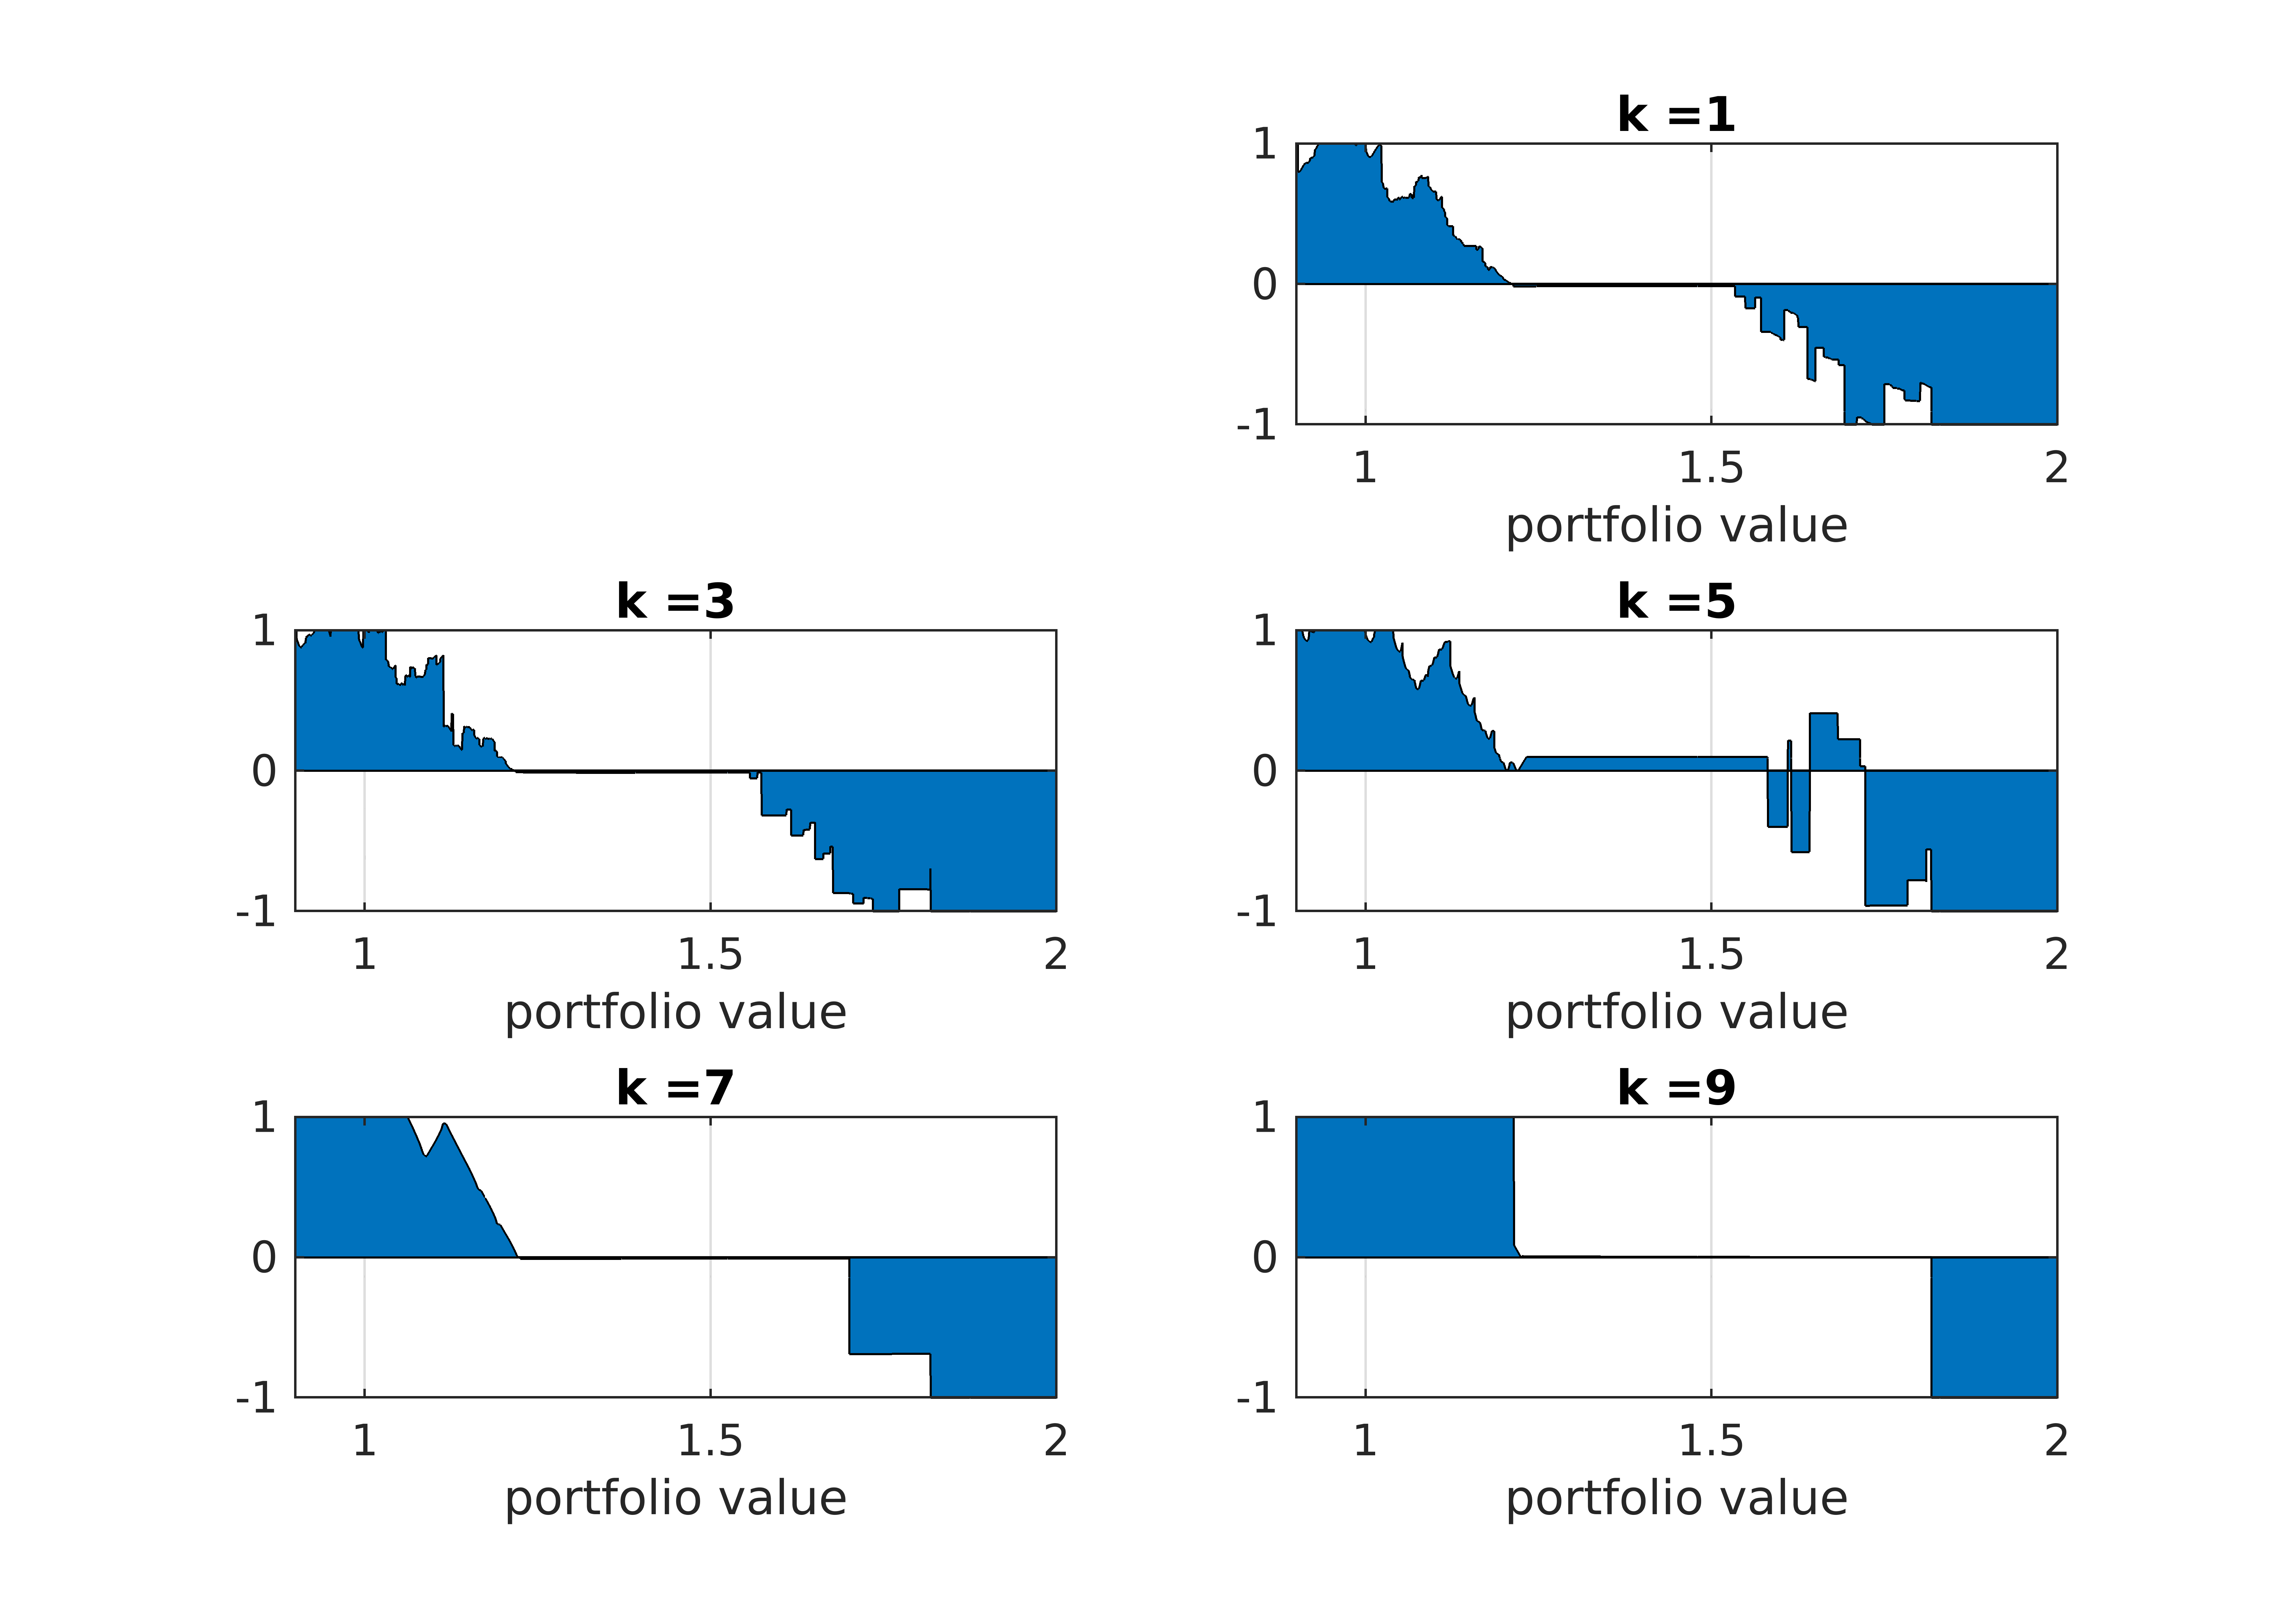
\includegraphics[scale = 0.8]{Images/mapsext1}}
	\caption{allocation maps}
	\label{fig:ext1_maps}
\end{figure}


\begin{figure}[h]
	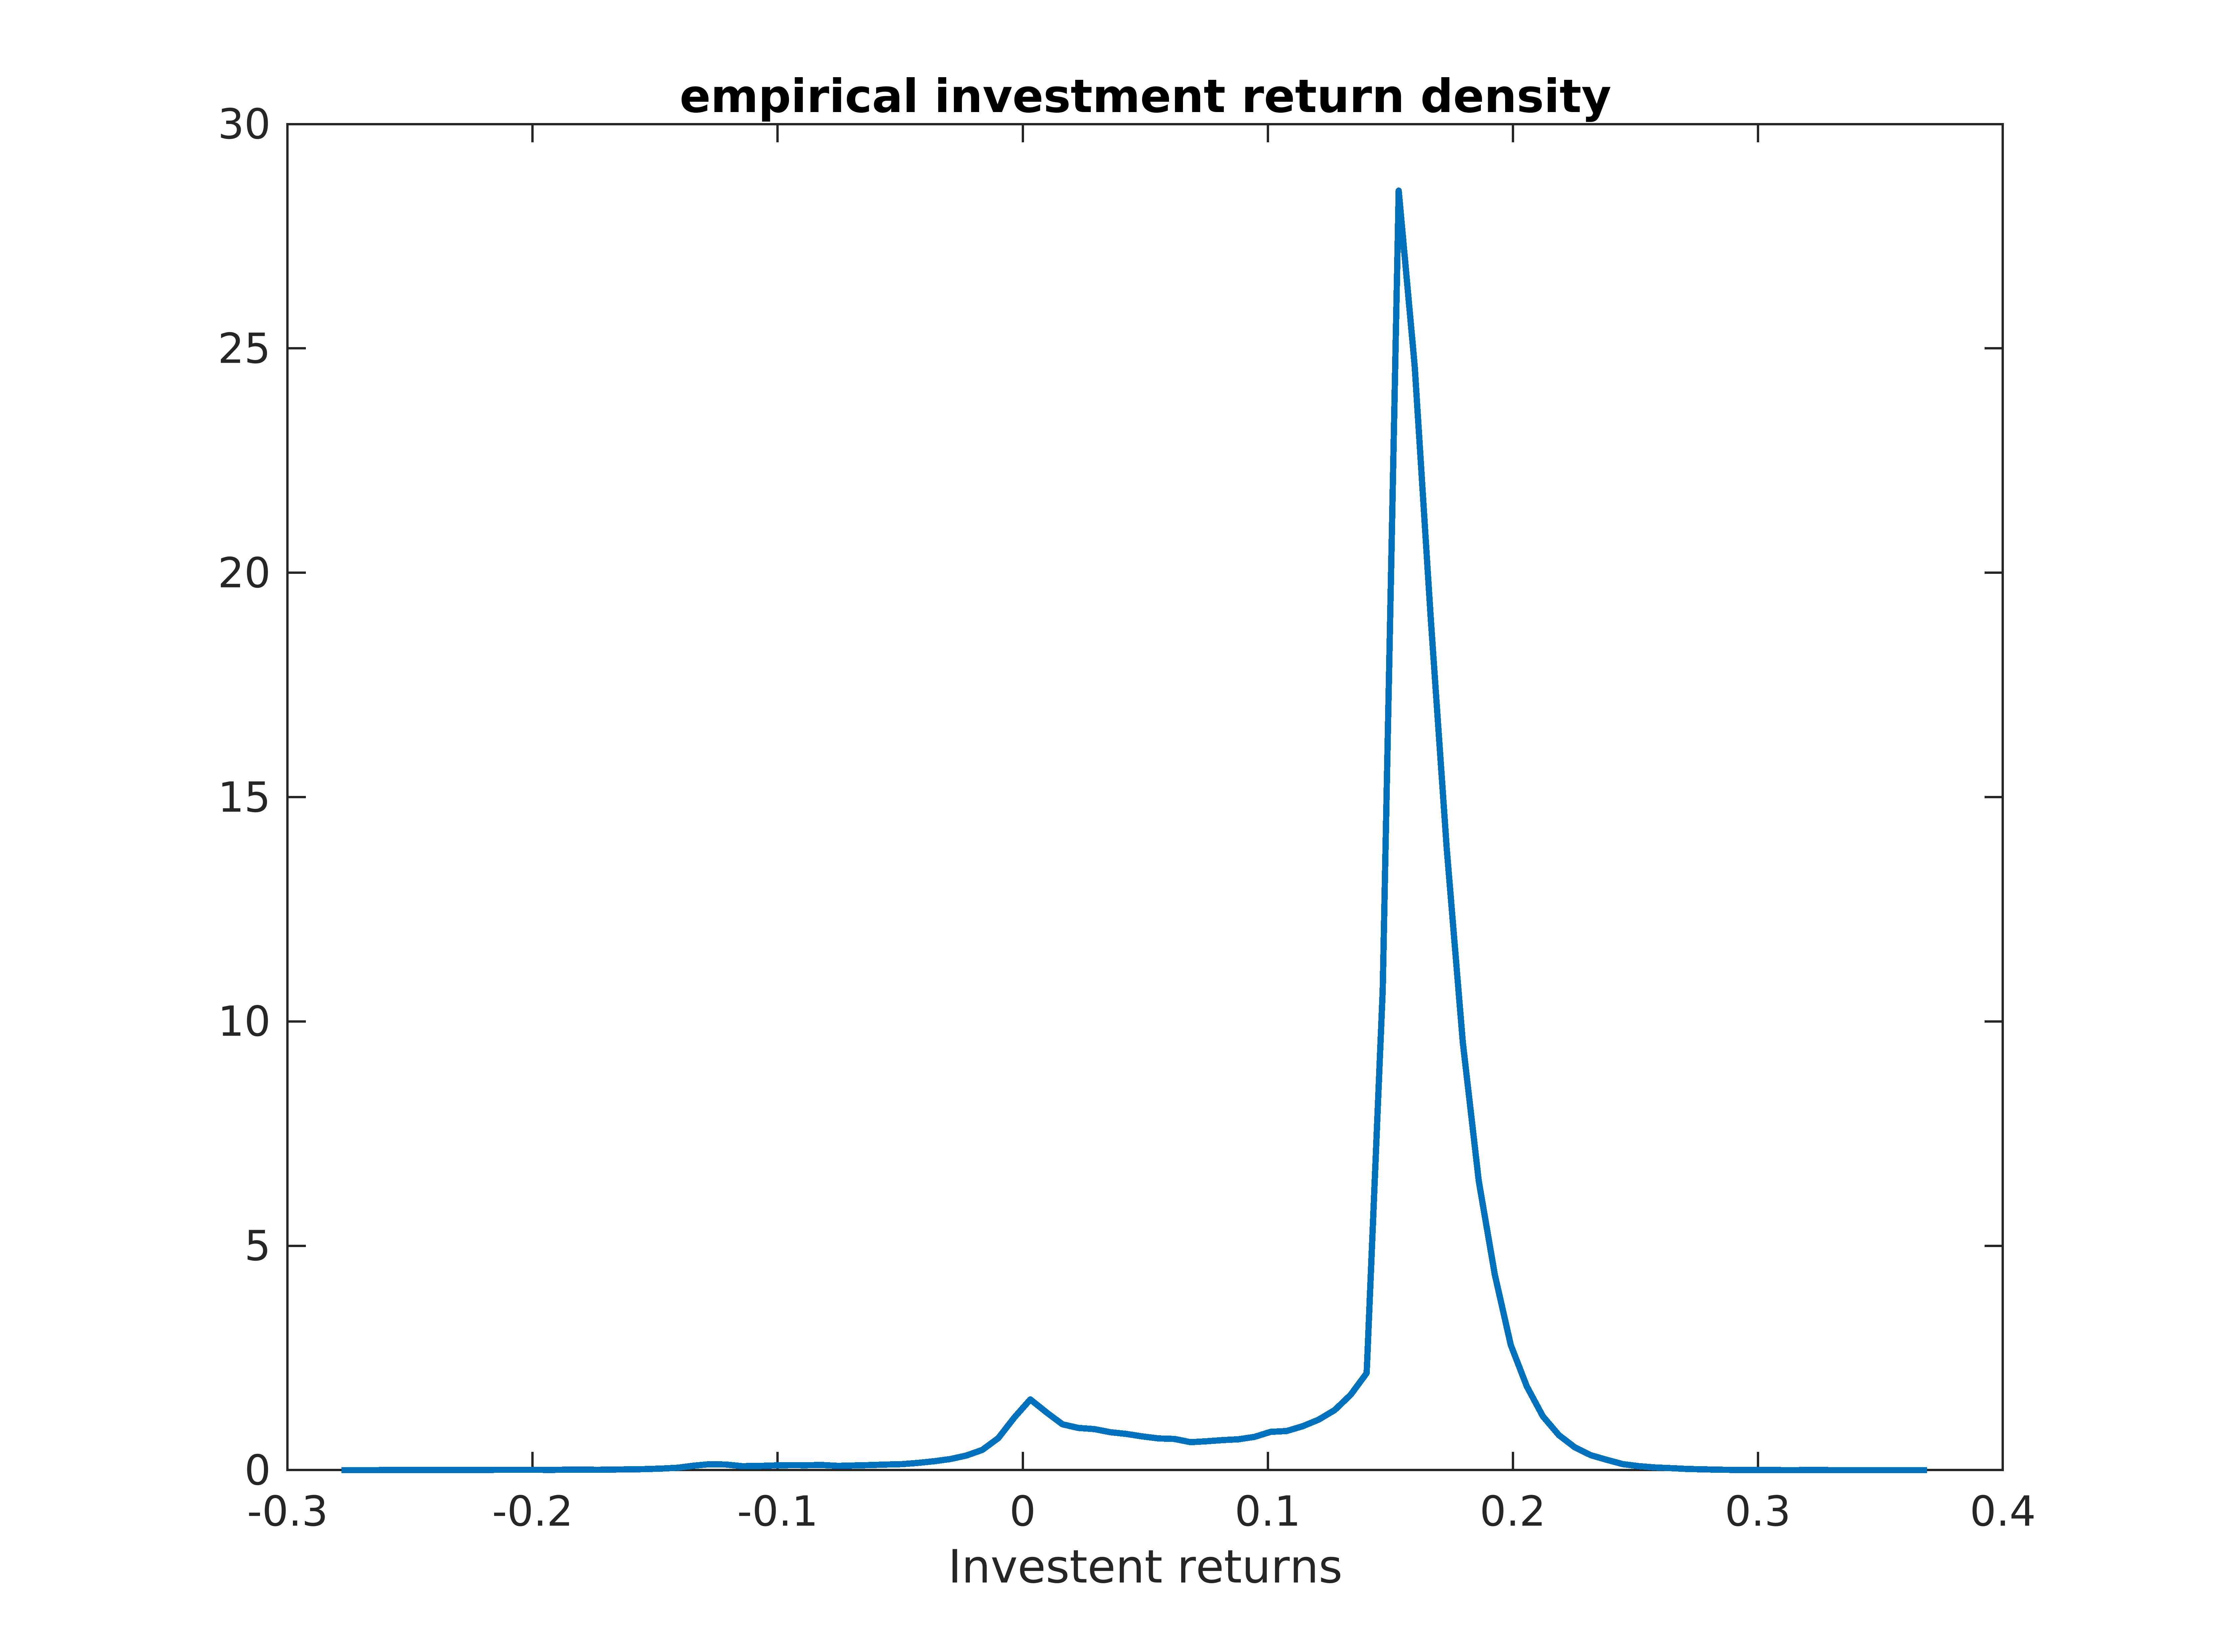
\includegraphics[scale = 0.5]{Images/Densityext1}
	\caption{Investment return empirical density function}
\end{figure}
\begin{wraptable}{l}{7cm}
		\begin{tabular}{@{}lc@{}}
			\toprule
			Statistics & value  \\
			%\addlinespace[0.5em]
			\midrule
			$p^{\star}$ & 0.9163\\
			\addlinespace[0.5em]	
			$p_{MC}$ & 0.9160\\
			\addlinespace[0.5em]
			Mean Return (ann) & 8.74\%\\
			\addlinespace[0.5em]
			Volatility (ann) & 5.07\%\\
			\addlinespace[0.5em]
			Median Return (ann) & 9.18\%\\
			\addlinespace[0.5em]
			Skewness & -3.43\\
			\addlinespace[0.5em]
			Kurtosis & 17.59\\
			\addlinespace[0.5em]
			Sharpe Ratio & 0.610\\
			\addlinespace[0.5em]
			Avg horizon [years] & 1.86 \\	
			\bottomrule
		\end{tabular}
		\caption{Investment performance obtained via Monte-Carlo simulation}
		\label{tab:performance_ext1}
\end{wraptable}

